\noindent{\small\textbf{CIÊNCIAS HUMANAS E SUAS TECNOLOGIAS}}

\noindent\textbf{Questões \ref{ch-first} a \ref{ch-last}} %arrumar o número


%
% História - Felipe
%

\questao \label{ch-first} %(Enem 2018)
\citacao{
A rebelião luso-brasileira em Pernambuco começou a ser urdida em 1644 e explodiu em 13 de junho de 1645, dia de Santo Antônio. Uma das primeiras medidas de João Fernandes foi decretar nulas as dívidas que os rebeldes tinham com os holandeses. Houve grande adesão da “nobreza da terra”, entusiasmada com esta proclamação heroica.}{
VAINFAS, R. Guerra declarada e paz fingida na restauração portuguesa. Tempo, n. 27, 2009.
}
O desencadeamento dessa revolta na América portuguesa seiscentista foi o resultado do(a)
\begin{alternativas}
\item fraqueza bélica dos protestantes batavos.
\item comércio transatlântico da África ocidental.
\item auxílio financeiro dos negociantes flamengos.
\item diplomacia internacional dos Estados ibéricos.
\item interesse econômico dos senhores de engenho.
\end{alternativas}

\questao %Enem 2016
\citacao{
A regulação das relações de trabalho compõe uma estrutura complexa, em que cada elemento se ajusta aos demais. A Justiça do Trabalho é apenas uma das peças dessa vasta engrenagem. A presença de representantes classistas na composição dos órgãos da Justiça do Trabalho é também resultante da montagem dessa regulação. O poder normativo também reflete essa característica. Instituída pela Constituição de 1934, a Justiça do Trabalho só vicejou no ambiente político do Estado Novo instaurado em 1937. }{
ROMITA, A. S. Justiça do Trabalho: produto do Estado Novo. In: PANDOLFI, D. (org.). Repensando o Estado Novo. Rio de Janeiro: FGV, 1999. }
A criação da referida instituição estatal na conjuntura histórica abordada teve por objetivo:
\begin{alternativas}
\item Legitimar os protestos fabris.
\item Ordenar os conflitos laborais. 
\item Oficializar os sindicatos plurais.
\item Assegurar os princípios liberais.
\item Unificar os salários profissionais.
\end{alternativas}

\questao %Enem 2014
\citacao{
A transferência da corte trouxe para a América portuguesa a família real e o governo da Metrópole. Trouxe também, e sobretudo, boa parte do aparato administrativo português. Personalidades diversas e funcionários régios continuaram embarcando para o Brasil atrás da corte, dos seus empregos e dos seus parentes após o ano de 1808. }{
NOVAIS, F. A.; ALENCASTRO, L. F. (Org.). História da vida privada no Brasil. São Paulo: Cia. das Letras, 1997. }
Os fatos apresentados se relacionam ao processo de independência da América portuguesa por terem 
\begin{alternativas}
\item incentivado o clamor popular por liberdade. 
\item enfraquecido o pacto de dominação metropolitana. 
\item motivado as revoltas escravas contra a elite colonial.
\item obtido o apoio do grupo constitucionalista português.
\item provocado os movimentos separatistas das províncias.
\end{alternativas}

\questao %Enem 2014
\citacao{
O problema central a ser resolvido pelo Novo Regime era a organização de outro pacto de poder que pudesse substituir o arranjo imperial com grau suficiente de estabilidade. O próprio presidente Campos Sales resumiu claramente seu objetivo: ``É de lá, dos estados, que se governa a República, por cima das multidões que tumultuam agitadas nas ruas da capital da União. A política dos estados é a política nacional''. }{
CARVALHO, J. M. Os Bestializados: o Rio de Janeiro e a República que não foi. São Paulo: Companhia das Letras, 1987 (adaptado).}
Nessa citação, o presidente do Brasil no período expressa uma estratégia política no sentido de
\begin{alternativas}
\item governar com a adesão popular.
\item ampliar a influência da capital no cenário nacional.
\item conferir maior autonomia às prefeituras.
\item democratizar o poder do governo central.
\item atrair o apoio das oligarquias regionais.
\end{alternativas}

\questao %Enem 2012
De acordo com um estudo recente, na Bahia, entre 1680 e 1797, de 160 filhas nascidas em 53 famílias de destaque, mais de 77\% foram enviadas a conventos, 5\% permaneceram solteiras e apenas 14 se casaram. Tendo em vista que, no período colonial, mesmo entre pessoas livres, a população masculina era maior que a feminina, esses dados sugerem que...
\begin{alternativas}
\item os senhores-de-engenho não deixavam suas filhas casarem com pessoas de nível social e econômico inferior. 
\item entre as mulheres ricas, a devoção religiosa era mais intensa e fervorosa do que entre as mulheres pobres. 
\item os homens brancos preferiam manter sua liberdade sexual a se submeterem ao despotismo dos senhores-de-engenho.
\item a vida na colônia era tão insuportável para as mulheres que elas preferiam vestir o hábito de freiras na Metrópole.
\item a sociedade colonial se pautava por padrões morais que privilegiavam o sexo e a beleza e não o status e a riqueza.
\end{alternativas}

\questao %Enem 2006
A moderna democracia brasileira foi construída entre saltos e sobressaltos. Em 1954, a crise culminou no suicídio do presidente Vargas. No ano seguinte, outra crise quase impediu a posse do presidente eleito, Juscelino Kubitschek. Em 1961, o Brasil quase chegou à guerra civil depois da inesperada renuncia do presidente Jânio Quadros. Três anos mais tarde, um golpe militar depôs o presidente João Goulart, e o país viveu durante vinte anos em regime autoritário. A partir dessas informações, relativas à historia republicana brasileira, assinale a opção correta:
\begin{alternativas}
\item Ao término do governo João Goulart, Juscelino Kubitschek foi eleito presidente da Republica. 
\item A renúncia de Jânio Quadros representou a primeira grande crise do regime republicano brasileiro. 
\item Apos duas décadas de governos militares, Getúlio Vargas foi eleito presidente em eleições diretas.
\item A trágica morte de Vargas determinou o fim da carreira política de João Goulart.
\item No período republicano citado, sucessivamente, um presidente morreu, um teve sua posse contestada, um renunciou e outro foi deposto.
\end{alternativas}

\questao %Enem 2004
Constituição de 1824: ``Art. 98. O Poder Moderador é a chave de toda a organização política, e é delegado privativamente ao Imperador (…) para que incessantemente vele sobre a manutenção da Independência, equilíbrio, e harmonia dos demais poderes políticos (...) dissolvendo a Câmara dos Deputados nos casos em que o exigir a salvação do Estado.'' 
Frei Caneca: ``O Poder Moderador da nova invenção maquiavélica é a chave mestra da opressão da nação brasileira e o garrote mais forte da liberdade dos povos. Por ele, o imperador pode dissolver a Câmara dos Deputados, que é a representante do povo, ficando sempre no gozo de seus direitos o Senado, que é o representante dos apaniguados do imperador.'' (Voto sobre o juramento do projeto de Constituição)\\
Para Frei Caneca, o Poder Moderador definido pela Constituição outorgada pelo Imperador em 1824 era
\begin{alternativas}
\item adequado ao funcionamento de uma monarquia constitucional, pois os senadores eram escolhidos pelo Imperador. 
\item eficaz e responsável pela liberdade dos povos, porque garantia a representação da sociedade nas duas esferas do poder legislativo. 
\item arbitrário, porque permitia ao Imperador dissolver a Câmara dos Deputados, o poder representativo da sociedade.
\item neutro e fraco, especialmente nos momentos de crise, pois era incapaz de controlar os deputados representantes da Nação.
\item capaz de responder às exigências políticas da nação, pois supria as deficiências da representação política.
\end{alternativas}

\questao %Enem 2020
\citacao{
Com efeito, até a destruição de Cartago, o povo e o Senado romano governavam a República em harmonia e sem paixão, e não havia entre os cidadãos luta por glória ou dominação; o medo do inimigo mantinha a cidade no cumprimento do dever. Mas, assim que o medo desapareceu dos espíritos, introduziram-se os males pelos quais a prosperidade tem predileção, isto é, a libertinagem e o orgulho.}{
SALÚSTIO. \textit{A conjuração de Catilina/A guerra de Jugurta.} Petrópolis: Vozes, 1990 (adaptado).}
O acontecimento histórico mencionado no texto de Salústio, datado de I a.C., manteve correspondência com o processo de 
\begin{alternativas}
\item demarcação de terras públicas.   
\item imposição da escravidão por dividas.   
\item restrição da cidadania por parentesco.   
\item restauração de instituições ancestrais.   
\item expansão das fronteiras extrapeninsulares. 
\end{alternativas}

\questao %Enem 2018
\citacao{
Temos vivido, como nação, atormentados pelos males modernos e pelos males do passado, pelo velho e pelo novo, sem termos podido conhecer uma história de rupturas revolucionárias. Não que não tenhamos nos modernizado e chegado ao desenvolvimento. Mas não eliminamos relações, estruturas e procedimentos contrários ao espírito do tempo. Nossa modernização tem sido conservadora.}{
NOGUEIRA, M. \textit{As possibilidades da política: ideias para a reforma democrática do Estado.} Rio de Janeiro: Paz e Terra, 1998.}
O texto apresenta uma análise recorrente sobre o processo de modernização do Brasil na segunda metade do século XX. De acordo com a análise, uma característica desse processo reside na(s)
\begin{alternativas}
\item uniformização técnica dos espaços de produção.    
\item construção municipalista do regime representativo.    
\item organização estadual das agremiações partidárias.    
\item limitações políticas no estabelecimento de reformas sociais.    
\item restrições financeiras no encaminhamento das demandas ruralistas. 
\end{alternativas}

\questao %Enem 2018
\citacao{Torna-se importante, portanto, salientar que as pautas econômicas dominantes não se incompatibilizavam com demandas políticas ou por garantia de direitos contra as decisões da própria Justiça do Trabalho. Pelo contrário, muitas greves incluíam várias demandas de natureza distinta, e mesmo em demandas primariamente econômicas, colocava-se muitas vezes a dimensão do enfrentamento político. Em todos esses casos, confirma-se a hipótese de que direitos instituídos ou garantias das convenções coletivas, respaldadas pela Justiça do Trabalho, não significavam conquistas materiais às quais os trabalhadores tivessem acesso líquido e certo. Era preciso muitas vezes recorrer às greves para garantir direitos conquistados.}{
MATTOS, M. B. Greves, sindicatos e repressão policial no Rio de Janeiro (1954-1964). \textit{Revista Brasileira de História}, n. 47, 2004 (adaptado).}
De acordo com o texto, um dos problemas com os quais as organizações sindicais de trabalhadores se defrontavam, de 1954 a 1964, era o descompasso entre
\begin{alternativas}
\item legislação e realidade social.    
\item profissão e formação técnica.    
\item meio rural e cidades industriais.    
\item população e representação parlamentar.    
\item empresariado nacional e capitais estrangeiros.
\end{alternativas}

%
% Geografia - Luis Felipe
%

\questao
O gráfico abaixo representa a relação entre o tamanho e a totalidade dos imóveis rurais no Brasil. Que característica da estrutura fundiária brasileira está evidenciada no gráfico apresentado?
\citacao{
\begin{center}
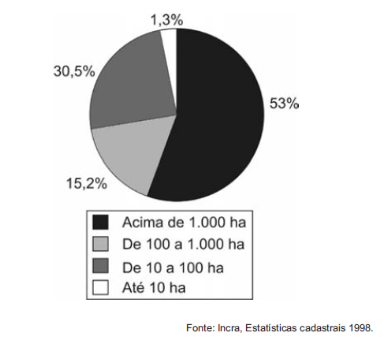
\includegraphics[trim= 0 45 55 0, clip, width=.8\columnwidth]{subareas/ciencias_humanas/geografia-1.png}
\end{center}
}{Fonte: Incra, Estatísticas cadastrais 1998.}
\begin{alternativas}
\item A concentração de terras nas mãos de poucos.
\item A existência de poucas terras agricultáveis.
\item O domínio territorial dos minifúndios.
\item A primazia da agricultura familiar.
\item A debilidade dos plantations modernos.
\end{alternativas}

\questao
\citacao{
\textbf{TEXTO I} – A nossa luta é pela democratização da propriedade da terra, cada vez mais concentrada em nosso país. Cerca de 1\% de todos os proprietários controla 46\% das terras. Fazemos pressão por meio da ocupação de latifúndios improdutivos e grandes propriedades, que não cumprem a função social, como determina a Constituição de 1988. Também ocupamos as fazendas que têm origem na grilagem de terras públicas.}{
Disponível em www.mst.org.br – acessado em 25 de agosto de 2011 (adaptado).}
\citacao{
\textbf{TEXTO II} – O pequeno proprietário rural é igual a um pequeno proprietário de loja: quanto menor o negócio, mais difícil de manter, pois tem que ser produtivo e os encargos são difíceis de custear. Sou a favor de propriedades produtivas e sustentáveis, que gerem empregos. Apoiar uma empresa produtiva que gere emprego é muito mais barato e gera muito mais do que apoiar a reforma agrária.}{
LESSA, C. Disponível em www.observatoriopolitico.org.br, acessado em 25 de agosto de 2011 (adaptado).}
Nos fragmentos dos textos, os posicionamentos em relação à reforma agrária se opõem. Isso acontece porque os autores associam a reforma agrária, respectivamente, à
\begin{alternativas}
\item Redução do inchaço urbano e à crítica ao minifúndio camponês.
\item Ampliação da renda nacional e à prioridade ao mercado externo.
\item Contestação da mecanização agrícola e ao combate ao êxodo rural.
\item Privatização de empresas estatais e ao estímulo ao crescimento econômico.
\item Correção de distorções históricas e ao prejuízo ao agronegócio.
\end{alternativas}

\questao
A dinâmica de transformação das cidades tende a apresentar como consequência a expansão das áreas periféricas pelo(a)
\begin{alternativas}
\item Direcionamento organizado do fluxo de pessoas, devido à existência de um grande número de serviços.
\item Delimitação de áreas para uma ocupação organizada do espaço físico, melhorando a qualidade de vida.
\item Crescimento descontrolado da população urbana e aumento da especulação imobiliária.
\item Implantação de políticas públicas que promovem a moradia e o direito à cidade aos seus moradores.
\item Reurbanização de moradias nas áreas centrais, mantendo o trabalhador próximo ao seu emprego, diminuindo os deslocamentos para a periferia.
\end{alternativas}

\questao
\citacao{
Subindo morros, margeando córregos ou penduradas em palafitas, as favelas fazem parte da paisagem de um terço dos municípios do país, abrigando mais de 10 milhões de pessoas, segundo dados do Instituto Brasileiro de Geografia e Estatística (IBGE).}{
MARTINS A. R. \textit{A favela como um espaço da cidade.}\\
Disponível em http://www.revistaescola.abril.com.br Acessado em 31 de julho de 2010. }
A situação das favelas no país reporta a graves problemas de desordenamento territorial. Nesse sentido, uma característica comum a esses espaços tem sido
\begin{alternativas}
\item O planejamento para a implantação de infraestruturas urbanas necessárias para atender às necessidades básicas dos moradores.
\item A organização de associações de moradores interessadas na melhoria do espaço urbano e financiadas pelo poder público.
\item A presença de ações referentes à educação ambiental com consequente preservação dos espaços naturais circundantes.
\item A ocupação de áreas de risco suscetíveis a enchentes ou desmoronamentos com consequentes perdas materiais e humanas.
\item O isolamento socioeconômico dos moradores ocupantes desses espaços com a resultante multiplicação de políticas que tentam reverter esse quadro.
\end{alternativas}

\questao
Leia a descrição de quatro grandes tipos climáticos do Brasil e, em seguida, examine o mapa, que representa a divisão regional do país em grandes tipos climáticos.\\
1. Chuvas escassas e irregulares, com precipitações médias de 500 a 700 mm, e temperaturas elevadas, com médias de 28 °C.\\
2. Chuvas entre 2 000 e 3 000 mm e elevadas temperaturas durante todo o ano, com médias de 26 °C.\\
3. Regular distribuição das chuvas durante o ano e temperaturas mais amenas, com médias inferiores a 18 °C e esporádica queda de neve.\\
4. Duas estações bem marcantes: uma chuvosa e quente, com 1 200 mm de precipitação e médias térmicas de 24 °C, e outra seca e fria, com 200 mm de chuvas e 17 °C de média térmica.\\
\citacao{
\begin{center}
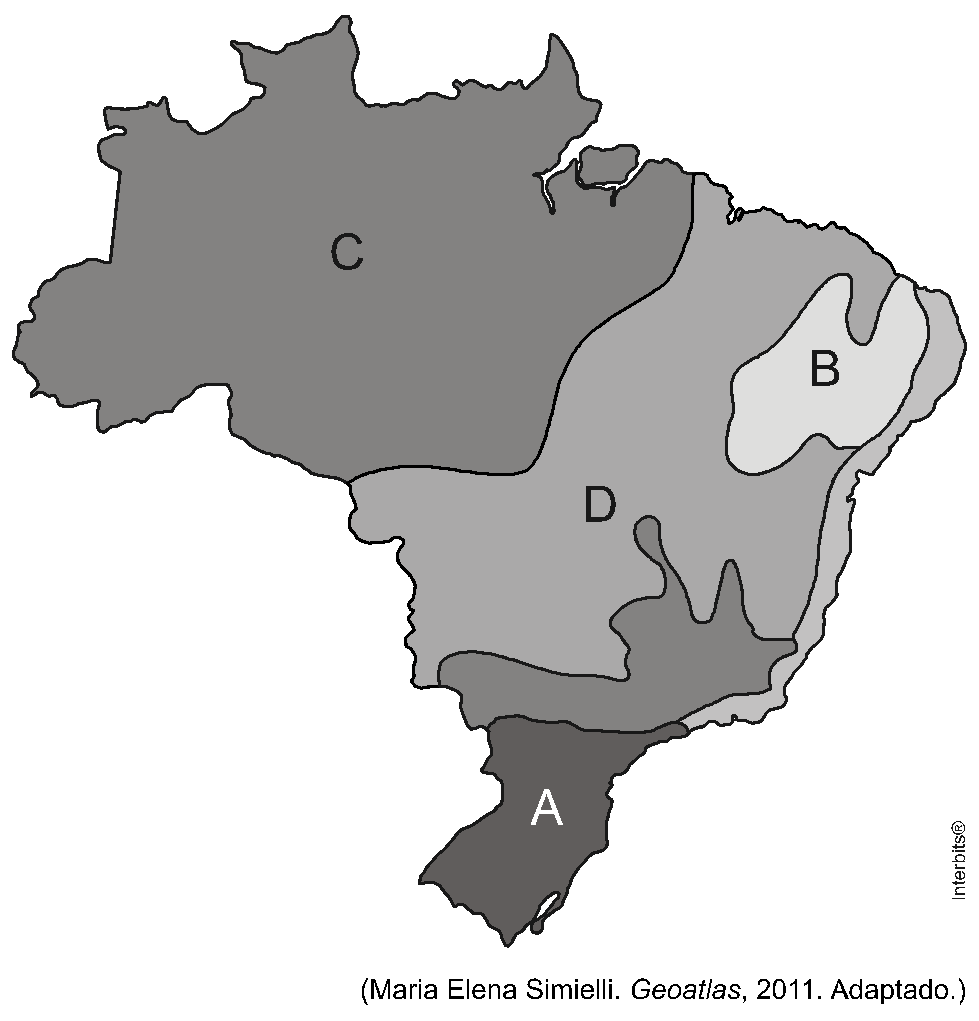
\includegraphics[trim= 0 45 0 0,
clip,width=\columnwidth]{subareas/ciencias_humanas/geografia-2.png}
\end{center}
}{
(Maria Elena Smielli. \textit{Geoatlas}, 2011. Adaptado)}
Assinale a alternativa que contém a correta associação entre a descrição climática e sua área de ocorrência.
\begin{alternativas}
\item 1B; 2C; 3A; 4D.   
\item 1C; 2A; 3B; 4D.   
\item 1B; 2A; 3D; 4C.   
\item 1A; 2C ; 3D; 4B.
\item 1C; 2B; 3D; 4A.
\end{alternativas}

\questao
Assinale a alternativa que indica corretamente as zonas climáticas indicadas abaixo:\\
I. Verões quentes e secos; vegetação com oliveiras e parreiras.\\
II. Quatro estações bem definidas; solos escuros e férteis; vegetação aciculifoliada.\\
III. Clima quente e úmido; solos expostos a laterização; vegetação densa e hidrófila.
\begin{alternativas}
\item I – Tropical; II – Polar; III – Equatorial.
\item I – Mediterrânea; II – Tropical; III – Equatorial.
\item I – Temperada; II – Semiárida; III – Polar.
\item I – Mediterrânea; II – Temperada; III – Tropical.
\item I – Equatorial;  II – Temperada; III – Tropical.
\end{alternativas}

\questao
{\itshape O fenômeno dos ``rios voadores''\\
``Rios voadores'' são cursos de água atmosféricos, invisíveis, que passam por cima de nossas cabeças transportando umidade e vapor de água da bacia Amazônica para outras regiões do Brasil. A floresta Amazônica funciona como uma bomba d’água. Ela ``puxa'' para dentro do continente umidade evaporada do oceano Atlântico que, ao seguir terra adentro, cai como chuva sobre a floresta. Pela ação da evapotranspiração da floresta, as árvores e o solo devolvem a água da chuva para a atmosfera na forma de vapor de água, que volta a cair novamente como chuva mais adiante. O Projeto Rios Voadores busca entender mais sobre a evapotranspiração da floresta Amazônica e a importante contribuição da umidade gerada por ela no regime de chuvas do Brasil.}\\
A partir da leitura do texto e da observação do mapa, é correto afirmar que, no Brasil,
\begin{alternativas}
\item cada vez mais, a floresta é substituída por agricultura ou pastagem, procedimento que promove o desenvolvimento econômico, sem influenciar, significativamente, o clima na América do Sul.   
\item a destruição da Amazônia, sobretudo pela expansão da pecuária e do cultivo de soja, pode alterar consideravelmente a produção de umidade e as chuvas na América do Sul, especialmente no sudeste brasileiro.
\item o atual desenvolvimento da Amazônia não afeta o sistema hidrológico, devido à aplicação de medidas rigorosas contra o desmatamento e danos à biodiversidade da floresta.   
\item os mecanismos climatológicos devem ser considerados na avaliação dos riscos decorrentes de ações como o desmatamento, as queimadas, a abertura de novas fronteiras agrícolas e a liberação dos gases do efeito estufa.   
\item a circulação atmosférica é dominada por massas de ar carregadas de umidade que, encontrando a barreira natural formada pelos Andes, precipitam-se na encosta leste, alimentando as bacias hidrográficas do país.
\end{alternativas}

\questao
\citacao{
{\itshape ``A chegada dos colonizadores, invadindo e ocupando o nosso continente – até aí chamado Aby ayala pelas populações indígenas -, representava a chegada de um novo modelo civilizatório, com o despojo das riquezas naturais dos nossos países, da destruição das populações indígenas e a introdução da pior das selvagerias: a escravidão. Chegaram com a espada e a cruz, para dominar e oprimir, para impor seu poder militar e tentar impor sua religião. (...) Durante mais de 4 séculos fomos reduzidos a isso. Os ciclos econômicos da nossa história foram determinados não por decisões das populações locais, mas das necessidades e interesses do mercado mundial, controlado pelas potências colonizadoras. Pau brasil, açúcar, café e borracha no nosso caso. Ouro, prata, cobre, carne, couro, e outras tantas riquezas do novo continente, foram sendo reiteradamente dilapidados em favor do enriquecimento das potências colonizadoras europeias.''}}{
– Emir Sader, Portal VioMundo (13/10/2011)}
Seguindo a lógica proposta pelo autor do fragmento apresentado, o desenvolvimento econômico do Brasil:
\begin{alternativas}
\item Foi autônomo, atendendo às demandas econômicas e sociais nacionais desde a época da colonização.
\item Já superou a influência histórica do domínio europeu, a exemplo do racismo e da exploração econômica, extintos.
\item Sempre atendeu às demandas impostas pelos interesses hegemônicos: primeiro da Europa, depois dos EUA e hoje, também, da China.
\item Foi influenciado pela colonização europeia apenas do ponto de vista econômico, uma vez que o desenvolvimento social contou somente com influências locais.
\item Só não foi bem sucedido pela insistente presença do Estado, que negou a autonomia do Brasil ao priorizar as políticas sociais ao invés dos investimentos econômicos.
\end{alternativas}

\questao
Sobre a globalização dos problemas ambientais é correto afirmar:\\
I - Após a Revolução Industrial, a Natureza passou a ser vista como uma fonte de recursos econômicos a ser explorada por meio de instrumentos cada vez mais sofisticados, criados pela ciência e pela tecnologia. Nesse processo, o meio ambiente foi submetido a uma contínua devastação, pondo em risco o equilíbrio do planeta e afetando a vida de toda a humanidade.\\
II - Nas últimas décadas do século XX, com o agravamento dos problemas ambientais, a sociedade se mobilizou para tentar deter os efeitos nocivos das atividades econômicas, predatórias e poluentes, porém os interesses financeiros continuam a se sobrepor à consciência ambiental.\\
III - Grupos ecológicos se multiplicaram e a pressão social resultou na aprovação pelos poderes públicos de leis de proteção ao meio ambiente, apesar de serem muitas vezes desrespeitadas.\\
IV - No âmbito internacional, a preservação do meio ambiente passou a constituir elemento importante de um país para negociar a comercialização de seus produtos e recebimento de empréstimos.\\
Estão corretas apenas as afirmações:
\begin{alternativas}
\item I e II.
\item II e III.
\item III e IV
\item I, III e IV.
\item I, II, III e IV.
\end{alternativas}

\questao
Ao analisar o avanço tecnológico ocorrido durante o processo de Globalização é correto afirmar:
\begin{alternativas}
\item Os avanços tecnológicos aconteceram de maneira simultânea em todo o planeta.
\item O setor de serviço perdeu espaço no mundo globalizado, enquanto a indústria “verde” ganhou terreno devido à pressão do movimento ecologista.
\item Observa-se uma tendência dos monopólios dos meios de comunicação asiáticos em detrimento das empresas americanas que dominavam o mercado.
\item O crescimento econômico dos países em desenvolvimento tornou-se uma realidade, pois agora o saber é difundido democraticamente através da internet.
\item Os fluxos de informações e capitais estão em crescente aumento, obedecendo a nova tendência tecnológica de um capitalismo informacional.
\end{alternativas}

%
% Sociologia Marina
%

\questao %Enem 2020
\citacao{
A propriedade compreende, em seu conteúdo e alcance, além do tradicional direito de uso, gozo e disposição por parte de seu titular, a obrigatoriedade do atendimento de sua função social, cuja definição é inseparável do requisito obrigatório do uso racional da propriedade e dos recursos ambientais que lhe são integrantes. O proprietário, como membro integrante da comunidade, se sujeita a obrigações crescentes que, ultrapassando os limites do direito de vizinhança, no âmbito do direito privado, abrangem o campo dos direitos da coletividade, visando o bem-estar geral, no âmbito do direito público.}{
JELINEK. R O princípio da função social da propriedade é sua repercussão sobre o sistema do Código Civil. Disponível em: www.mp.rs.gov.br. Acesso em 20 fev. 2013}
Os movimentos em prol da reforma agrária, que atuam com base no conceito de direito à
propriedade apresentado no texto, propõem-se a
\begin{alternativas}
\item Reverter o processo de privatização fundiária.
\item Ressaltar a inviabilidade da produção latifundiária.
\item Defender a desapropriação dos espaços improdutivos.
\item Impedir a produção exportadora nas terras agricultáveis.
\item Coibir o funcionamento de empresas agroindustriais no campo.
\end{alternativas}

\questao %Enem 2017
\citacao{
No Brasil, assim como em vários outros países, os modernos movimentos LGBT representam um desafio às formas de condenação e perseguição social contra desejos e comportamentos sexuais anticonvencionais associados à vergonha, imoralidade, pecado, degeneração, doença. Falar do movimento LGBT implica, portanto, chamar a atenção para a sexualidade como fonte de estigmas, intolerância, opressão.
}{
SIMÕES, J. Homossexualidade e movimento LGBT: estigma, diversidade e cidadania. In: BOTELHO, A.; SCHWARCZ, L. M. Cidadania, um projeto em construção. São Paulo: Claro Enigma, 2012 (adaptado).}
O movimento social abordado justifica-se pela defesa do direito de
\begin{alternativas}
\item Organização sindical.
\item Participação partidária.
\item Manifestação religiosa.
\item Formação profissional.
\item Afirmação identitária.
\end{alternativas}

\questao %Enem 2015
\citacao{
Ninguém nasce mulher: torna-se mulher. Nenhum destino biológico, psíquico, econômico define a forma que a fêmea humana assume no seio da sociedade; é o conjunto da civilização que elabora esse produto intermediário entre o macho e o castrado que qualificam o feminino.}{
BEAUVOIR, S. O segundo sexo. Rio de Janeiro: Nova Fronteira, 1980.}
Na década de 1960, a proposição de Simone de Beauvoir contribuiu para estruturar um movimento social que teve como marca o(a)
\begin{alternativas}
\item Ação do Poder Judiciário para criminalizar a violência sexual.
\item Pressão do Poder Legislativo para impedir a dupla jornada de trabalho.
\item Organização de protestos públicos para garantir a igualdade de gênero.
\item Oposição de grupos religiosos para impedir os casamentos homoafetivos.
\item Estabelecimento de políticas governamentais para promover ações afirmativas.
\end{alternativas}

\questao %Enem 2020 - Digital
\citacao{
A masculinidade, assim como a feminilidade, é uma construção histórica e cultural. Em nossa cultura, a dança caracteriza-se, no sentido geral, como um universo predominantemente feminino. Homens que dançam são geralmente considerados homossexuais, por não se enquadrarem dentro das normas culturais hegemônicas de gênero e sexualidade. Por outro lado, demonstram a não existência de um único tipo de masculinidade, enfatizando que as identidades humanas são múltiplas e plurais. No contexto da dança, as representações hegemônicas de gênero e as regulações sociais que essas impõem não se manifestam deforma igual em todas as modalidades de dança. Persiste essa forte representação cultural ocidental que associa o balé à feminilidade e à homossexualidade. Em outras danças, ela não se revela tão forte, e os homens não aparecem em menor número, como nas tradicionais danças folclóricas ou no moderno hip hop.}{
ANDREOLI, G. S. Representações de masculinidade na dança contemporânea. Movimento, n. 1, 2011 (adaptado).}
\begin{alternativas}
\item padronização da inserção dos homens nessas manifestações corporais.
\item identificação de como essas práticas regulam uma única masculinidade.
\item reconhecimento das diferentes masculinidades.
\item contestação das normas sociais pelo balé.
\item reforço de uma feminilidade hegemônica.
\end{alternativas}

\questao
\textbf{TEXTO I}
\citacao{
\begin{center}
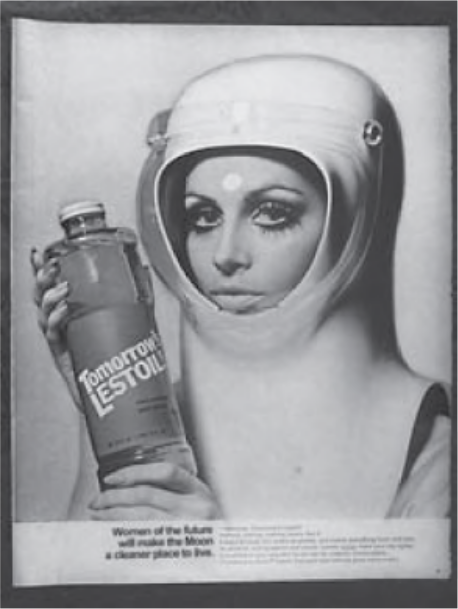
\includegraphics[width=\columnwidth]{subareas/ciencias_humanas/sociologia-1.png}
\textbf{Tradução: ``As mulheres do futuro farão da Lua um lugar mais limpo para se viver''}
\end{center}
}{
Disponível em: www.propagandashistoricas.com.br. Acesso em: 16 out. 2015.}
\textbf{TEXTO II}
\citacao{
\begin{center}
\textbf{Metade da nova equipe da Nasa é composta por mulheres} 
\end{center}
Até hoje, cerca de 350 astronautas americanos já estiveram no espaço, enquanto as mulheres não chegam a ser um terço desse número. Após o anúncio da turma composta 50\% por mulheres, alguns internautas escreveram comentários machistas e desrespeitosos sobre a escolha nas redes sociais.}{
Disponível em: https://catracalivre.com.br. Acesso em: 10 mar. 2016}
A comparação entre o anúncio publicitário de 1968 e a repercussão da notícia de 2016 mostra a:
\begin{alternativas}
\item elitização da carreira científica.
\item qualificação da atividade doméstica.
\item ambição de indústrias patrocinadoras.
\item manutenção de estereótipos de gênero.
\item equiparação de papéis nas relações familiares.
\end{alternativas}

\questao %Enem 2014
\citacao{
O cidadão norte-americano desperta num leito construído segundo padrão originário do Oriente Próximo, mas modificado na Europa Setentrional antes de ser transmitido à América. Sai debaixo de cobertas feitas de algodão cuja planta se tornou doméstica na Índia. No restaurante, toda uma série de elementos tomada de empréstimo o espera. O prato é feito de uma espécie de cerâmica inventada na China. A faca é de aço, liga feita pela primeira vez na Índia do Sul; o garfo é inventado na Itália medieval; a colher vem de um original romano. Lê notícias do dia impressas em caracteres inventados pelos antigos semitas, em material inventado na China e por um processo inventado na Alemanha.}{
LINTON, R. \textit{O homem: uma introdução à antropologia.} São Paulo: Martins, 1959 (adaptado)}
A situação descrita é um exemplo de como os costumes resultam da:
\begin{alternativas}
\item assimilação de valores de povos exóticos.
\item experimentação de hábitos sociais variados.
\item recuperação de heranças da Antiguidade Clássica.
\item fusão de elementos de tradições culturais diferentes.
\item valorização de comportamento de grupos privilegiados.
\end{alternativas}

\questao %Enem 2011
\citacao{
A Lei 10.639, de 9 de janeiro de 2003, inclui no currículo dos estabelecimentos de ensino fundamental e médio, oficiais e particulares, a obrigatoriedade do ensino sobre História e Cultura Afro-Brasileira e determina que o conteúdo programático incluirá o estudo da História da África e dos africanos, a luta dos negros no Brasil, a cultura negra brasileira e o negro na formação da sociedade nacional, resgatando a contribuição do povo negro nas áreas social, econômica e política pertinentes à História do Brasil, além de instituir, no calendário escolar, o dia 20 de novembro como data comemorativa do ``Dia da Consciência Negra''.}{
Disponível em: http://www.planalto.gov.br. Acesso em: 27 jul. 2010
(adaptado).}
A referida lei representa um avanço não só para a educação nacional, mas também para a sociedade brasileira, porque
\begin{alternativas}
\item Legitima o ensino das ciências humanas nas escolas.
\item Divulga conhecimentos para a população afro-brasileira.
\item Reforça a concepção etnocêntrica sobre a África e sua cultura.
\item Garante aos afrodescendentes a igualdade no acesso à educação.
\item Impulsiona o reconhecimento da pluralidade étnicoracial do país.
\end{alternativas}

\questao %Enem 2018
\citacao{
Num país que conviveu com o trabalho escravo durante quatro séculos, o trabalho doméstico é ainda considerado um subemprego. E os indivíduos que atuam nessa área são, muitas vezes, vistos pelos patrões como um mal necessário: é preciso ter em casa alguém que limpe o banheiro, lave a roupa, tire o pó e arrume a gaveta. Existe uma inegável desvalorização das atividades domésticas em relação a outros tipos de trabalho.}{
RANGEL, C. Domésticas: nascer, deixar, permanecer ou simplesmente estar. In: SOUZA, E. (Org.). \textbf{Negritude, cinema e educação.} Belo Horizonte: Mazza, 2011 (adaptado).}
Objeto de legislação recente, o enfrentamento do problema mencionado resultou na
\begin{alternativas}
\item criação de novos ofícios.
\item ampliação de direitos sociais.
\item redução da desigualdade de gênero.
\item fragilização da representação sindical.
\item erradicação da atividade informal.
\end{alternativas}

\questao %Enem PPL 2016
\textbf{TEXTO I}
\citacao{
\begin{verse}
Cidadão\\
Tá vendo aquele edifício, moço?\\
Ajudei a levantar\\
Foi um tempo de aflição\\
Eram quatro condução\\
Duas pra ir, duas pra voltar\\
Hoje depois dele pronto\\
Olho pra cima e fico tonto\\
Mas me vem um cidadão\\
E me diz desconfiado\\
“Tu tá aí admirado\\
Ou tá querendo roubar?”\\
Meu domingo tá perdido\\
Vou pra casa entristecido\\
Dá vontade de beber\\
E pra aumentar meu tédio\\
Eu nem posso olhar pro prédio\\
Que eu ajudei a fazer.\\
\end{verse}}{
BARBOSA. L. In: ZÉ RAMALHO, 20 Super Sucessos. Rio de Janeiro: Sony Music. 1999 - fragmento}
\textbf{TEXTO II}
\citacao{
O trabalhador fica mais pobre à medida que produz mais riqueza e sua produção cresce em força e extensão. O trabalhador torna-se uma mercadoria ainda mais barata à medida que cria mais bens. Esse fato simplesmente subentende que o objeto produzido pelo trabalho, o seu produto, agora se lhe opõe como um ser estranho, como uma força independente do produtor.}{
MARX, K. Manuscritos econômicos-filosóficos (Os Primeiros). São Paulo: Boitempo Editorial, 2004}
Com base nos textos. a relação entre trabalho e modo de produção capitalista é:
\begin{alternativas}
\item Baseada na desvalorização do trabalho especializado e no aumento da demanda social por novos postos de emprego.
\item Fundada no crescimento proporcional entre o número de trabalhadores e o aumento da produção de bens e serviços.
\item Estruturada na distribuição equânime de renda e no declínio do capitalismo industrial e tecnocrata.
\item Instaurada a partir do fortalecimento da luta de classes e da criação da economia solidária.
\item Derivada do aumento da riqueza e da ampliação da exploração do trabalhador.
\end{alternativas}

\questao %Enem PPL 2013
\citacao{
O servo pertence à terra e rende frutos ao dono da terra. O operário urbano livre, ao contrário, vende-se a si mesmo e, além disso, por partes. Vende em leilão 8,10,12,15 horas da sua vida, dia após dia, a quem melhor pagar, ao proprietário das matérias-primas, dos instrumentos de trabalho e dos meios de subsistência, isto é, ao capitalista.}{
MARX, K. Trabalho assalariado e capital \& salário, preço e lucro. São Paulo: Expressão
Popular, 2010}
O texto indica que houve uma transformação dos espaços urbanos e rurais com a implementação do sistema capitalista, devido às mudanças tecnossociais ligadas ao:
\begin{alternativas}
\item Desenvolvimento agrário e ao regime de servidão.
\item Aumento da produção rural, que fixou a população nesse meio.
\item Desenvolvimento das zonas urbanas e às novas relações de trabalho.
\item Aumento populacional das cidades associado ao regime de servidão.
\item Desenvolvimento da produção urbana associada às relações servis de trabalho.
\end{alternativas}

%
% Filosofia - Rafael
%

\questao
\citacao{
Alguns dos desejos são naturais e necessários; outros, naturais e não necessários; outros, nem naturais nem necessários, mas nascidos de vã opinião. Os desejos que não nos trazem dor se não satisfeitos não são necessários, mas o seu impulso pode ser facilmente desfeito, quando é difícil obter sua satisfação ou parecem geradores de dano.}{
EPICURO DE SAMOS. ``Doutrinas principais''. In: SANSON, V. F. Textos de filosofia. Rio de Janeiro: Eduff, 1974.}
No fragmento da obra filosófica de Epicuro, o homem tem como fim
\begin{alternativas}
\item defender a indiferença e a impossibilidade de se atingir o saber.
\item valorizar os deveres e as obrigações sociais.
\item alcançar o prazer moderado e a felicidade.
\item aceitar o sofrimento e o rigorismo da vida com resignação.
\end{alternativas}

\questao
\citacao{
Uma norma só deve pretender validez quando todos os que possam ser concernidos por ela cheguem (ou possam chegar), enquanto participantes de um discurso prático, a um acordo quanto à validade dessa norma.}{
HABERMAS, J. Consciência moral e agir comunicativo. Rio de Janeiro: Tempo Brasileiro, 1989.}
Segundo Habermas, a validez de uma norma deve ser estabelecida pelo(a):
\begin{alternativas}
\item técnica científica, que aumenta o poder do homem.
\item razão comunicativa, que requer um consenso.
\item liberdade humana, que consagra a vontade.
\item poder político, que se concentra no sistema partidário.
\item conhecimento filosófico, que expressa a verdade.
\end{alternativas}

\questao
\citacao{
Compreende-se assim o alcance de uma reivindicação que surge desde o nascimento da cidade na Grécia antiga: a redação das leis. Ao escrevê-las, não se faz mais que assegurar-lhes permanência e fixidez. As leis tornam-se bem comum, regra geral, suscetível de ser aplicada a todos da mesma maneira.}{
VERNANT, J. P. As origens do pensamento grego. Rio de Janeiro: Bertrand Brasil, 1992 (adaptado).}
Para o autor, a reivindicação atendida na Grécia antiga, ainda vigente no mundo contemporâneo, buscava garantir o seguinte princípio:
\begin{alternativas}
\item Tripartição — separação entre os poderes políticos estatais.
\item Isonomia — igualdade de tratamento aos cidadãos.
\item Elegibilidade — permissão para candidatura aos cargos públicos.
\item Equiparação — igualdade de gênero na participação política.
\item Transparência — acesso às informações governamentais.
\end{alternativas}

\questao
\citacao{
Hoje, a indústria cultural assumiu a herança civilizatória da democracia de pioneiros e empresários, que tampouco desenvolvera uma fineza de sentido para os desvios espirituais. Todos são livres para dançar e para se divertir, do mesmo modo que, desde a neutralização histórica da religião, são livres para entrar em qualquer uma das inúmeras seitas. Mas a liberdade de escolha de ideologia, que reflete sempre a coerção econômica, revela-se em todos os setores como a liberdade de escolher o que é sempre a mesma coisa.}{
ADORNO, T; HORKHEIMER, M. A dialética do esclarecimento: fragmentos filosóficos. Rio de Janeiro: Zahar, 1995.}
A liberdade de escolha na civilização ocidental, de acordo com a análise do texto, é um(a):
\begin{alternativas}
\item legado social.
\item ilusão da contemporaneidade.
\item produto da moralidade.
\item conquista da humanidade.
\item patrimônio político.
\end{alternativas}

\questao
\citacao{
Sentimos que toda satisfação de nossos desejos advinda do mundo assemelha-se à esmola que mantém hoje o mendigo vivo, porém prolonga amanhã a sua fome. A resignação, ao contrário, assemelha-se à fortuna herdada: livra o herdeiro para sempre de todas as preocupações.}{
SCHOPENHAUER, A. Aforismo para a sabedoria da vida. São Paulo: Martins Fontes, 2005.} O trecho destaca uma ideia remanescente de uma tradição filosófica ocidental, segundo a qual a felicidade se mostra indissociavelmente ligada à
\begin{alternativas}
\item fugacidade do conhecimento empírico.
\item consagração de relacionamentos afetivos.
\item administração da independência interior.
\item liberdade de expressão religiosa.
\item busca de prazeres efêmeros.
\end{alternativas}

\questao
\citacao{
Nunca nos tornaremos matemáticos, por exemplo, embora nossa memória possua todas as demonstrações feitas por outros, se nosso espírito não for capaz de resolver toda espécie de problemas; não nos tornaríamos filósofos, por ter lido todos os raciocínios de Platão e Aristóteles, sem poder formular um juízo sólido sobre o que nos é proposto. Assim, de fato, pareceríamos ter aprendido, não ciências, mas histórias.}{
DESCARTES, R. Regras para a orientação do espírito. São Paulo: Martins Fontes, 1999.}
Em busca pelo saber verdadeiro, o autor considera o conhecimento, de modo crítico, como resultado da
\begin{alternativas}
\item investigação da natureza empírica.
\item retomada da tradição intelectual.
\item imposição de valores ortodoxos.
\item autonomia do sujeito pensante.
\item liberdade do agente moral.
\end{alternativas}

\questao
\textbf{TEXTO I}
\citacao{Fragmento B91: Não se pode banhar duas vezes no mesmo rio, nem substância mortal alcança duas vezes a mesma condição; mas pela intensidade e rapidez da mudança, dispersa e de novo reúne.}{
HERÁCLITO. Fragmentos (Sobre a natureza) São Paulo: Abril Cultural, 1996 (adaptado).}
\textbf{TEXTO II}
\citacao{
Fragmento B8: São muitos os sinais de que o ser é ingênito e indestrutível, pois é compacto, inabalável sem fim; não foi nem será, pois é agora um todo homogêneo, uno, contínuo.}{
PARMÊNIDES. Da natureza. São Paulo: Loyola, 2002 (adaptado).}
Os fragmentos do pensamento pré-socrático expõem uma oposição que se insere no
campo das
\begin{alternativas}
\item investigações do pensamento sistemático.
\item preocupações do período mitológico.
\item discussões de base ontológica.
\item habilidade da retórica sofística.
\item verdades do mundo sensível.
\end{alternativas}

\questao
\citacao{
A arte pré-histórica africana foi incontestavelmente um veículo de mensagens pedagógicas e sociais. Os San, que constituem hoje um povo mais próximo da realidade das representações rupestres, afirmam que seus antepassados lhes explicaram sua visão do mundo a partir desse gigantesco livro que são as galerias. A educação dos povos que desconhecem a escrita está baseada sobretudo na imagem e no som, no audiovisual.}{
KI-ZERBO, J. A arte pré-histórica africana. In: KI-ZERBO, J. (Org.) História geral da África. Brasília: Unesco, 2010.}
De acordo com o texto, a arte mencionada é importante para os povos que a cultivam por colaborar para o(a)
\begin{alternativas}
\item expansão da propriedade individual.
\item surgimento dos laços familiares.
\item rejeição de práticas exógenas.
\item transmissão dos saberes acumulados.
\item ruptura da disciplina hierárquica.
\end{alternativas}

\questao
\citacao{
Montaigne deu o nome para um novo gênero literário; foi dos primeiros a instituir na literatura moderna um espaço privado, o espaço do “eu”, do texto íntimo. Ele cria um novo processo de escrita filosófica, no qual hesitações, autocríticas, correções entram no próprio texto.}{
COELHO, M. Montaigne. São Paulo: Publifolha, 2001 (adaptado).}
O novo gênero de escrita aludido no texto é o(a)
\begin{alternativas}
\item diálogo, que discute assuntos com diferentes interlocutores.
\item carta, que comunica informações para um conhecido.
\item confissão, que relata experiências de transformação.
\item meditação, que propõe preparações para o conhecimento.
\item ensaio, que expõe concepções subjetivas de um tema.
\end{alternativas}

\questao \label{ch-last}
\citacao{
\begin{center}
Declaração de Salamanca – 1994
\end{center}
Acreditamos e proclamamos que: toda criança tem direito fundamental à educação e deve ser dada a oportunidade de atingir e manter o nível adequado de aprendizagem; toda criança possui características, interesses, habilidades e necessidades de aprendizagem que são únicas; sistemas educacionais deveriam ser designados e programas educacionais deveriam ser implementados no sentido de se levar em conta a vasta diversidade de tais características e necessidades.}{
Disponível em: http://portal.mec.gov.br Acesso em: 4 out. 2015.}
Como signatário da Declaração citada, o Brasil comprometeu-se com a elaboração de políticas públicas educacionais que contemplem a
\begin{alternativas}
\item criação de privilégios.
\item valorização da meritocracia.
\item pluralidade dos sujeitos.
\item contenção dos gastos.
\item padronização do currículo.
\end{alternativas}